\documentclass{article}

% content/resources/templates/preamble.tex
\usepackage[margin=0.6in]{geometry}
\author{Milav Dabgar}
\usepackage{amsmath,amssymb,amsthm}
\usepackage{booktabs}
\usepackage{multirow}
\usepackage{xcolor}
\usepackage{tcolorbox}
\tcbuselibrary{breakable,skins}
\usepackage[colorlinks=true,linkcolor=blue]{hyperref}
\usepackage{titlesec}
\usepackage{enumitem}
\usepackage{tikz}
\usepackage{pgfplots}
\usepackage{circuitikz}
\usepackage[version=4]{mhchem}
\usepackage{longtable}
\usepackage{array}
\usepackage{float}
\usepackage{caption}
\usepackage{listings}

\lstset{
  basicstyle=\small\ttfamily,
  breaklines=true,
  breakatwhitespace=false,
  postbreak=\mbox{\textcolor{red}{$\hookrightarrow$}\space},
  float=false,
  numbers=left,
  numberstyle=\tiny\color{gray},
  numbersep=10pt,
  xleftmargin=2em,
  keywordstyle=\color{blue},
  commentstyle=\color{green!60!black},
  stringstyle=\color{purple},
  backgroundcolor=\color{gray!5},
  showstringspaces=false,
  tabsize=2,
  captionpos=b,
  keepspaces=true,
  columns=flexible
}

\pgfplotsset{compat=1.18}
\usetikzlibrary{shapes,arrows,positioning,calc,patterns,decorations.pathmorphing,decorations.markings,arrows.meta}

% Color scheme
\definecolor{headcolor}{RGB}{0,102,204}
\definecolor{keycolor}{RGB}{220,20,60}
\definecolor{solutioncolor}{RGB}{34,139,34}
\definecolor{mnemoniccolor}{RGB}{148,0,211}
\definecolor{codecolor}{RGB}{0,0,100}

% Spacing
\setlength{\parskip}{3pt}
\setlist[itemize]{nosep}
\setlist[enumerate]{nosep}

% Title formatting
\titleformat{\section}{\Large\bfseries\color{headcolor}}{\thesection}{1em}{}
\titleformat{\subsection}{\large\bfseries\color{headcolor}}{\thesubsection}{1em}{}

% Pandoc tightlist compatibility
\providecommand{\tightlist}{%
  \setlength{\itemsep}{0pt}\setlength{\parskip}{0pt}}

% Pandoc longtable compatibility
\newcounter{none}
\def\thenone{}


% content/resources/templates/english-boxes.tex

% Custom environments
\newtcolorbox{solutionbox}{
 breakable,
 enhanced,
 colback=solutioncolor!5!white,
 colframe=solutioncolor!75!black,
 fonttitle=\bfseries,
 title=Solution
}

\newtcolorbox{solutionboxnobreak}{
 colback=solutioncolor!5!white,
 colframe=solutioncolor!75!black,
 fonttitle=\bfseries,
 title=Solution
}

\newtcolorbox{keyformula}{
 breakable,
 enhanced,
 colback=keycolor!5!white,
 colframe=keycolor!75!black,
 fonttitle=\bfseries,
 title=Key Formula
}

\newtcolorbox{mnemonicboxenv}{
 breakable,
 enhanced,
 colback=mnemoniccolor!5!white,
 colframe=mnemoniccolor!75!black,
 fonttitle=\bfseries,
 title=Mnemonic
}

\newcommand{\mnemonicbox}[1]{%
  \begin{mnemonicboxenv}
    #1
  \end{mnemonicboxenv}
}


% Custom commands for GTU solutions
% This file defines semantic commands for consistent formatting

% Question command with automatic formatting
\newcommand{\question}[2]{%
  \section*{Question #1}%
  \textbf{#2}%
}

% OR question variant
\newcommand{\questionor}[2]{%
  \section*{Question #1 OR}%
  \textbf{#2}%
}

% Proper table environment with caption
\newenvironment{answertable}[1]{%
  \begin{table}[htbp]
  \centering
  \caption{#1}
}{%
  \end{table}
}

% Proper figure environment for diagrams
\newenvironment{answerdiagram}[1]{%
  \begin{figure}[htbp]
  \centering
  \caption{#1}
}{%
  \end{figure}
}

% Semantic markup for key terms
\newcommand{\keyword}[1]{\textbf{#1}}
\newcommand{\code}[1]{\texttt{#1}}
\newcommand{\classname}[1]{\texttt{#1}}
\newcommand{\methodname}[1]{\texttt{#1}}

% Proper quotation marks
\newcommand{\mnemonic}[1]{``#1''}


\title{Modern Physics (DI01000061) - Winter 2024 Solution}
\date{January 9, 2025}

\begin{document}
\maketitle

\questionmarks{1}{14}{Fill in the blanks / MCQs}

\begin{solutionbox}
\begin{center}
\captionof{table}{MCQ Answers}
\begin{tabulary}{\linewidth}{|C|L|C|L|}
\hline
\textbf{No.} & \textbf{Answer} & \textbf{No.} & \textbf{Answer} \\ \hline
(1) & (a) Si & (8) & (b) 0.5 Hz \\ \hline
(2) & (a) 1.50 & (9) & (a) 300000 km/s \\ \hline
(3) & (b) greater than & (10) & (b) solid \\ \hline
(4) & (c) 4 & (11) & (a) crest and trough \\ \hline
(5) & (d) Total internal reflection & (12) & (b) monochromatic \\ \hline
(6) & (d) frequency & (13) & (a) Single mode \\ \hline
(7) & (a) Coulomb & (14) & (b) 45\textdegree \\ \hline
\end{tabulary}
\end{center}
\end{solutionbox}

\begin{mnemonicbox}
\mnemonic{Silicon Glass Bridge Optic Frequency Coulomb Hz Solid Crest Mono Single 45}
\end{mnemonicbox}

\questionmarks{2(A)}{6}{Attempt any two}

\questionmarks{2(A)(1)}{3}{Differentiate between accuracy and precision.}

\begin{solutionbox}
\begin{center}
\captionof{table}{Accuracy vs Precision}
\begin{tabulary}{\linewidth}{|L|L|L|}
\hline
\textbf{Parameter} & \textbf{Accuracy} & \textbf{Precision} \\ \hline
Definition & Closeness to true value & Consistency of repeated measurements \\ \hline
Focus & Correctness & Reproducibility \\ \hline
Error Type & Systematic error & Random error \\ \hline
Example & Hitting bullseye & Hitting same spot repeatedly \\ \hline
\end{tabulary}
\end{center}

\begin{itemize}
    \item \keyword{Accuracy}: How close measurement is to actual value
    \item \keyword{Precision}: How close repeated measurements are to each other
\end{itemize}
\end{solutionbox}

\begin{mnemonicbox}
\mnemonic{Accurate Aims Actual, Precise Repeats Reliably}
\end{mnemonicbox}

\questionmarks{2(A)(2)}{3}{Determine the diameter of a sphere measured by micrometer screw, main scale reading is 5 mm and 50th division of circular scale is coinciding with base line. The least count of this instrument is 0.01 mm.}

\begin{solutionbox}
\textbf{Given:}
\begin{itemize}
    \item Main Scale Reading (MSR) = 5 mm
    \item Circular Scale Reading (CSR) = 50 divisions
    \item Least Count (LC) = 0.01 mm
\end{itemize}

\textbf{Formula:}
\[ \text{Total Reading} = \text{MSR} + (\text{CSR} \times \text{LC}) \]

\textbf{Calculation:}
\begin{align*}
\text{Total Reading} &= 5 + (50 \times 0.01) \\
&= 5 + 0.5 \\
&= 5.5 \text{ mm}
\end{align*}

\textbf{Diameter of sphere = 5.5 mm}
\end{solutionbox}

\begin{mnemonicbox}
\mnemonic{Main Scale Reading + Circular * Least Count}
\end{mnemonicbox}

\questionmarks{2(A)(3)}{3}{Calculate the amount of electric charge stored on either plate of a capacitor of capacitance 4 $\mu$F when connected across 12 volt battery.}

\begin{solutionbox}
\textbf{Given:}
\begin{itemize}
    \item Capacitance ($C$) = 4 $\mu$F = $4 \times 10^{-6}$ F
    \item Voltage ($V$) = 12 V
\end{itemize}

\textbf{Formula:}
\[ Q = CV \]

\textbf{Calculation:}
\begin{align*}
Q &= 4 \times 10^{-6} \times 12 \\
Q &= 48 \times 10^{-6} \text{ C} \\
Q &= 48 \ \mu\text{C}
\end{align*}

\textbf{Electric charge stored = 48 $\mu$C}
\end{solutionbox}

\begin{mnemonicbox}
\mnemonic{Charge equals Capacitance times Voltage}
\end{mnemonicbox}

\questionmarks{2(B)}{8}{Attempt any two}

\questionmarks{2(B)(1)}{4}{Draw a sketch of micrometer screw gauge with proper nomenclature.}

\begin{solutionbox}
\begin{center}
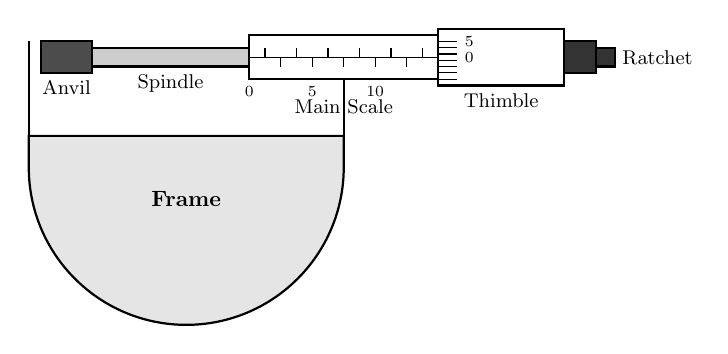
\begin{tikzpicture}[x=1cm, y=1cm, scale=0.8, transform shape]
    % Frame
    \draw[thick, fill=gray!20] (0,0) arc (180:360:2.5) -- (5,0) -- (5,0.5) -- (0,0.5) -- cycle;
    \draw[thick, fill=gray!20] (0,0.5) -- (0,2);
    \draw[thick, fill=gray!20] (5,0.5) -- (5,2);
    
    % Anvil
    \draw[thick, fill=black!70] (0.2,1.5) rectangle (1,2);
    \node[below, font=\small] at (0.6,1.5) {Anvil};

    % Spindle
    \draw[thick, fill=gray!40] (3.5,1.6) rectangle (1,1.9);
    \node[below, font=\small] at (2.25,1.6) {Spindle};

    % Sleeve/Main Scale
    \draw[thick, fill=white] (3.5,1.4) rectangle (6.5,2.1);
    \draw (3.5,1.75) -- (6.5,1.75); % Baseline
    \foreach \x in {3.5, 4.0, ..., 6.0}
        \draw (\x, 1.75) -- (\x, 1.6);
    \foreach \x in {3.75, 4.25, ..., 6.25}
        \draw (\x, 1.75) -- (\x, 1.9);
    \node[below, font=\scriptsize] at (3.5,1.4) {0};
    \node[below, font=\scriptsize] at (4.5,1.4) {5};
    \node[below, font=\scriptsize] at (5.5,1.4) {10};
    \node[below, font=\small] at (5,1.2) {Main Scale};

    % Thimble
    \draw[thick, fill=white] (6.5,1.3) rectangle (8.5,2.2);
    \foreach \y in {1.4, 1.5, ..., 2.1}
        \draw (6.5,\y) -- (6.8,\y);
    \node[right, font=\scriptsize] at (6.8,1.75) {0};
    \node[right, font=\scriptsize] at (6.8,2.0) {5};
    \node[below, font=\small] at (7.5,1.3) {Thimble};

    % Ratchet
    \draw[thick, fill=black!80] (8.5,1.5) rectangle (9,2);
    \draw[thick, fill=black!80] (9,1.6) rectangle (9.3,1.9);
    \node[right, font=\small] at (9.3,1.75) {Ratchet};

    % Labels
    \node[font=\bfseries] at (2.5,-0.5) {Frame};
\end{tikzpicture}
\captionof{figure}{Micrometer Screw Gauge}
\end{center}

\textbf{Main Components:}
\begin{itemize}
    \item \keyword{Frame}: U-shaped structure providing support
    \item \keyword{Anvil}: Fixed jaw for placing object
    \item \keyword{Spindle}: Movable screw mechanism
    \item \keyword{Thimble Scale}: Circular scale with 50 divisions
    \item \keyword{Main Scale}: Linear scale in mm
    \item \keyword{Ratchet}: For consistent pressure application
\end{itemize}
\end{solutionbox}

\begin{mnemonicbox}
\mnemonic{Frame Anvil Spindle Thimble Main Ratchet}
\end{mnemonicbox}

\questionmarks{2(B)(2)}{4}{Explain the zero, positive and negative errors for vernier calipers with proper diagram and list necessary steps to remove these types of errors.}

\begin{solutionbox}
\textbf{Types of Errors:}
\begin{center}
\captionof{table}{Vernier Caliper Errors}
\begin{tabulary}{\linewidth}{|L|L|L|}
\hline
\textbf{Error Type} & \textbf{Condition} & \textbf{Reading} \\ \hline
Zero Error & Zero line of vernier doesn't coincide with main scale zero & Non-zero reading when jaws closed \\ \hline
Positive Error & Vernier zero is right of main scale zero & Add correction \\ \hline
Negative Error & Vernier zero is left of main scale zero & Subtract correction \\ \hline
\end{tabulary}
\end{center}

\textbf{Diagrams:}
\begin{center}
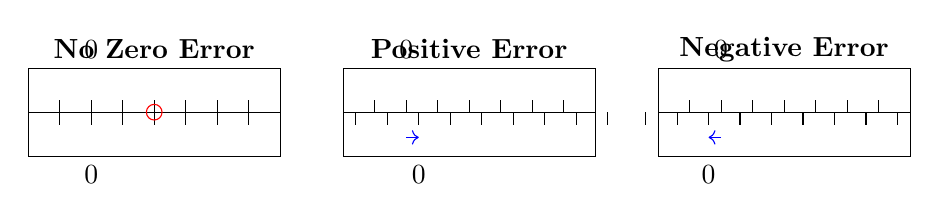
\begin{tikzpicture}[scale=0.8]
    % Zero Error
    \node[font=\bfseries] at (2, 2.5) {No Zero Error};
    \draw (0,1.5) rectangle (4,2.2); % Main
    \foreach \x in {0,0.5,...,4} \draw (\x,1.5) -- (\x,1.7);
    \node[above] at (1,2.2) {0};
    \draw (0,0.8) rectangle (4,1.5); % Vernier
    \foreach \x in {0,0.5,...,4} \draw (\x,1.5) -- (\x,1.3);
    \node[below] at (1,0.8) {0};
    \node at (2, 1.5) [draw, circle, red, inner sep=2pt] {};

    % Positive Error
    \node[font=\bfseries] at (7, 2.5) {Positive Error};
    \draw (5,1.5) rectangle (9,2.2); % Main
    \foreach \x in {5,5.5,...,9} \draw (\x,1.5) -- (\x,1.7);
    \node[above] at (6,2.2) {0};
    \draw (5,0.8) rectangle (9,1.5); % Vernier
    \foreach \x in {5,5.5,...,9} \draw (\x+0.2,1.5) -- (\x+0.2,1.3); % Shifted right
    \node[below] at (6.2,0.8) {0};
    \draw[->, blue] (6,1.1) -- (6.2,1.1);

    % Negative Error
    \node[font=\bfseries] at (12, 2.5) {Negative Error};
    \draw (10,1.5) rectangle (14,2.2); % Main
    \foreach \x in {10,10.5,...,14} \draw (\x,1.5) -- (\x,1.7);
    \node[above] at (11,2.2) {0};
    \draw (10,0.8) rectangle (14,1.5); % Vernier
    \foreach \x in {10,10.5,...,14} \draw (\x-0.2,1.5) -- (\x-0.2,1.3); % Shifted left
    \node[below] at (10.8,0.8) {0};
    \draw[->, blue] (11,1.1) -- (10.8,1.1);
\end{tikzpicture}
\captionof{figure}{Vernier Caliper Zero Errors}
\end{center}

\textbf{Steps to Remove Errors:}
\begin{itemize}
    \item \keyword{Check zero error} before measurement
    \item \keyword{Apply correction} to final reading
    \item \keyword{Clean jaws} regularly to prevent debris
    \item \keyword{Handle carefully} to avoid mechanical damage
\end{itemize}
\end{solutionbox}

\begin{mnemonicbox}
\mnemonic{Check Clean Correct Carefully}
\end{mnemonicbox}

\questionmarks{2(B)(3)}{4}{In an experiment of finding the periodic time of a simple pendulum, the observations are 1.96 s, 1.98 s, 2.00 s, 2.02 s, 2.04 s. Calculate absolute error, mean absolute error, relative error and percentage error.}

\begin{solutionbox}
\textbf{Data:} 1.96, 1.98, 2.00, 2.02, 2.04 s

\textbf{Calculations:}

1. \textbf{Mean value}:
\[ \bar{x} = \frac{1.96 + 1.98 + 2.00 + 2.02 + 2.04}{5} = \frac{10.00}{5} = 2.00 \text{ s} \]

2. \textbf{Absolute errors} ($|\Delta x_i| = |x_i - \bar{x}|$):
\begin{itemize}
    \item $|1.96 - 2.00| = 0.04$ s
    \item $|1.98 - 2.00| = 0.02$ s
    \item $|2.00 - 2.00| = 0.00$ s
    \item $|2.02 - 2.00| = 0.02$ s
    \item $|2.04 - 2.00| = 0.04$ s
\end{itemize}

3. \textbf{Mean absolute error}:
\[ \overline{\Delta x} = \frac{0.04 + 0.02 + 0.00 + 0.02 + 0.04}{5} = \frac{0.12}{5} = 0.024 \text{ s} \]

4. \textbf{Relative error}:
\[ \delta x = \frac{\overline{\Delta x}}{\bar{x}} = \frac{0.024}{2.00} = 0.012 \]

5. \textbf{Percentage error}:
\[ \% \text{ Error} = 0.012 \times 100 = 1.2\% \]

\textbf{Results:} Mean absolute error = 0.024 s, Relative error = 0.012, Percentage error = 1.2\%
\end{solutionbox}

\begin{mnemonicbox}
\mnemonic{Mean Absolute Relative Percentage}
\end{mnemonicbox}

\questionmarks{3(A)}{6}{Attempt any two}

\questionmarks{3(A)(1)}{3}{Define: Electric flux, Electric field, Potential Difference}

\begin{solutionbox}
\begin{center}
\captionof{table}{Definitions}
\begin{tabulary}{\linewidth}{|L|L|C|L|}
\hline
\textbf{Term} & \textbf{Definition} & \textbf{Unit} & \textbf{Formula} \\ \hline
Electric Flux & Number of electric field lines passing through a surface & Nm$^2$/C & $\Phi = E \cdot A$ \\ \hline
Electric Field & Force per unit positive charge & N/C & $E = F/q$ \\ \hline
Potential Difference & Work done per unit charge between two points & Volt & $V = W/q$ \\ \hline
\end{tabulary}
\end{center}

\begin{itemize}
    \item \keyword{Electric flux}: Measure of field lines penetrating surface
    \item \keyword{Electric field}: Region where electric force acts on charges
    \item \keyword{Potential difference}: Energy difference per unit charge
\end{itemize}
\end{solutionbox}

\begin{mnemonicbox}
\mnemonic{Flux Field Force, Work Watts Volts}
\end{mnemonicbox}

\questionmarks{3(A)(2)}{3}{Derive the formula for equivalent capacitance when three different capacitors are connected in series with necessary circuit diagram.}

\begin{solutionbox}
\textbf{Circuit Diagram:}
\begin{center}
\begin{tikzpicture}
    \draw (0,0) to[battery1, l=$V$] (0,2) -- (1,2)
        to[C, l=$C_1$] (2.5,2)
        to[C, l=$C_2$] (4,2)
        to[C, l=$C_3$] (5.5,2) -- (6.5,2) -- (6.5,0) -- (0,0);
\end{tikzpicture}
\captionof{figure}{Capacitors in Series}
\end{center}

\textbf{Derivation:}
\begin{itemize}
    \item \keyword{Same charge} $Q$ flows through each capacitor.
    \item \keyword{Voltage divides}: $V = V_1 + V_2 + V_3$
    \item For each capacitor: $V_1 = Q/C_1, V_2 = Q/C_2, V_3 = Q/C_3$
    \item Total voltage:
    \[ V = \frac{Q}{C_1} + \frac{Q}{C_2} + \frac{Q}{C_3} = Q \left( \frac{1}{C_1} + \frac{1}{C_2} + \frac{1}{C_3} \right) \]
    \item For equivalent capacitor $C_s$: $V = Q/C_s$
    \item Comparing equations:
    \[ \frac{1}{C_s} = \frac{1}{C_1} + \frac{1}{C_2} + \frac{1}{C_3} \]
\end{itemize}

\textbf{Formula:}
\[ \frac{1}{C_s} = \frac{1}{C_1} + \frac{1}{C_2} + \frac{1}{C_3} \]
\end{solutionbox}

\begin{mnemonicbox}
\mnemonic{Series Sums reciprocals, Same charge Splits voltage}
\end{mnemonicbox}

\questionmarks{3(A)(3)}{3}{Define: Infrasonic sound, Audible Sound, Ultrasonic sound}

\begin{solutionbox}
\begin{center}
\captionof{table}{Sound Classifications}
\begin{tabulary}{\linewidth}{|L|L|L|L|}
\hline
\textbf{Sound Type} & \textbf{Frequency Range} & \textbf{Characteristics} & \textbf{Applications} \\ \hline
Infrasonic & Below 20 Hz & Inaudible to humans & Earthquake detection \\ \hline
Audible & 20 Hz to 20 kHz & Audible to humans & Communication, music \\ \hline
Ultrasonic & Above 20 kHz & Inaudible to humans & Medical imaging, SONAR \\ \hline
\end{tabulary}
\end{center}

\begin{itemize}
    \item \keyword{Infrasonic}: Low frequency sounds below human hearing
    \item \keyword{Audible}: Normal hearing range for humans
    \item \keyword{Ultrasonic}: High frequency sounds above human hearing
\end{itemize}
\end{solutionbox}

\begin{mnemonicbox}
\mnemonic{Infra-Below, Audible-Between, Ultra-Above}
\end{mnemonicbox}

\questionmarks{3(B)}{8}{Attempt any two}

\questionmarks{3(B)(1)}{4}{Prove $C = \epsilon_0 A/d$ for parallel plate capacitor.}

\begin{solutionbox}
\textbf{Diagram:}
\begin{center}
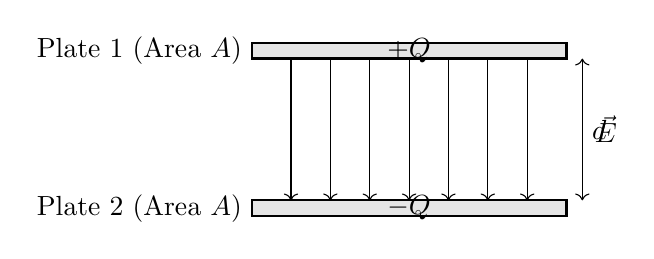
\begin{tikzpicture}
    % Plate 1
    \draw[thick, fill=gray!20] (0, 2) rectangle (4, 2.2);
    \node at (2, 2.1) {$+Q$};
    \node[left] at (0, 2.1) {Plate 1 (Area $A$)};
    
    % Plate 2
    \draw[thick, fill=gray!20] (0, 0) rectangle (4, 0.2);
    \node at (2, 0.1) {$-Q$};
    \node[left] at (0, 0.1) {Plate 2 (Area $A$)};
    
    % Field Lines
    \foreach \x in {0.5, 1.0, ..., 3.5}
        \draw[->] (\x, 2) -- (\x, 0.2);
    \node at (4.5, 1.1) {$\vec{E}$};
    
    % Distance
    \draw[<->] (4.2, 0.2) -- (4.2, 2);
    \node[right] at (4.2, 1.1) {$d$};
\end{tikzpicture}
\captionof{figure}{Parallel Plate Capacitor}
\end{center}

\textbf{Derivation:}
\begin{itemize}
    \item \keyword{Electric field} between plates: $E = \sigma/\epsilon_0 = Q/(\epsilon_0 A)$
    \item \keyword{Potential difference}: $V = E \times d = Qd/(\epsilon_0 A)$
    \item \keyword{Capacitance definition}: $C = Q/V$
    \item Substituting $V$:
    \[ C = \frac{Q}{Qd/(\epsilon_0 A)} = \frac{\epsilon_0 A}{d} \]
\end{itemize}

\textbf{Final Formula:}
\[ C = \frac{\epsilon_0 A}{d} \]

Where:
\begin{itemize}
    \item $\epsilon_0$: Permittivity of free space
    \item $A$: Area of plates
    \item $d$: Distance between plates
\end{itemize}
\end{solutionbox}

\begin{mnemonicbox}
\mnemonic{Capacitance equals epsilon-zero Area over distance}
\end{mnemonicbox}

\questionmarks{3(B)(2)}{4}{List the characteristics of electric field lines.}

\begin{solutionbox}
\textbf{Key Characteristics:}
\begin{enumerate}
    \item \keyword{Direction}: Start from positive charge and end at negative charge.
    \item \keyword{Density}: The closeness of lines indicates field strength (denser = stronger).
    \item \keyword{Continuous}: They are continuous curves without breaks in a charge-free region.
    \item \keyword{Non-intersecting}: Two field lines never cross each other (otherwise there would be two directions of field at one point).
    \item \keyword{Perpendicular}: They are always normal to the surface of a charged conductor.
    \item \keyword{Closed loops}: They do not form closed loops (electrostatic field is conservative).
    \item \keyword{Tangent}: Tangent to the line at any point gives the direction of the electric field.
\end{enumerate}
\end{solutionbox}

\begin{mnemonicbox}
\mnemonic{Positive to Negative, Dense means Strong, Never cross, Always perpendicular}
\end{mnemonicbox}

\questionmarks{3(B)(3)}{4}{Describe working and construction of magnetostriction method used for production of ultrasonic waves.}

\begin{solutionbox}
\textbf{Construction:}
\begin{center}
\begin{tikzpicture}[node distance=1.5cm, auto]
    \node [gtu block] (osc) {AC Oscillator};
    \node [gtu block, right=1cm of osc] (coil) {Coil};
    \node [gtu block, right=1cm of coil] (rod) {Nickel Rod};
    \node [gtu block, right=1cm of rod] (horn) {Horn};
    
    \path [gtu arrow] (osc) -- (coil);
    \path [gtu arrow] (coil) -- node[above] {Magnetic Field} (rod);
    \path [gtu arrow] (rod) -- node[above] {Vibrations} (horn);
    \path [gtu arrow] (horn) -- node[above] {Ultrasonic Waves} +(3,0);
\end{tikzpicture}
\captionof{figure}{Magnetostriction Oscillator Block Diagram}
\end{center}

\textbf{Components:}
\begin{itemize}
    \item \keyword{Nickel rod}: Ferromagnetic material showing magnetostriction effect.
    \item \keyword{Coil}: Solenoid wrapped around the rod to produce magnetic field.
    \item \keyword{AC oscillator}: Source of high-frequency alternating current.
    \item \keyword{Horn}: To transmit acoustic energy efficiently.
\end{itemize}

\textbf{Working Principle:}
\begin{itemize}
    \item When \keyword{AC current} flows through the coil, a rapidly changing \keyword{magnetic field} is produced.
    \item The ferromagnetic rod undergoes \keyword{magnetostriction} (change in length) at twice the frequency of the applied AC.
    \item This produces \keyword{mechanical vibrations} in the rod.
    \item If the frequency matches the natural frequency of the rod, resonance occurs, producing high-intensity \keyword{ultrasonic waves}.
\end{itemize}
\end{solutionbox}

\begin{mnemonicbox}
\mnemonic{AC Coil Makes Nickel vibrate, Creates Ultrasonic}
\end{mnemonicbox}

\questionmarks{4(A)}{6}{Attempt any two}

\questionmarks{4(A)(1)}{3}{A radio station broadcasts its radio signals at $9.26 \times 10^7$ Hz. Find the wavelength if the waves travel at a speed of $3.00 \times 10^8$ m/s.}

\begin{solutionbox}
\textbf{Given:}
\begin{itemize}
    \item Frequency ($f$) = $9.26 \times 10^7$ Hz
    \item Speed ($c$) = $3.00 \times 10^8$ m/s
\end{itemize}

\textbf{Formula:}
\[ c = f\lambda \implies \lambda = \frac{c}{f} \]

\textbf{Calculation:}
\begin{align*}
\lambda &= \frac{3.00 \times 10^8}{9.26 \times 10^7} \\
\lambda &= \frac{300}{92.6} \times 10^0 \\
\lambda &\approx 3.24 \text{ m}
\end{align*}

\textbf{Wavelength = 3.24 m}
\end{solutionbox}

\begin{mnemonicbox}
\mnemonic{Speed equals frequency times wavelength}
\end{mnemonicbox}

\questionmarks{4(A)(2)}{3}{State the Snell's law and explain refractive index of media.}

\begin{solutionbox}
\textbf{Snell's Law:}
The ratio of the sine of the angle of incidence to the sine of the angle of refraction is a constant value for a given pair of media.
\[ n_1 \sin \theta_1 = n_2 \sin \theta_2 \]
Where:
\begin{itemize}
    \item $n_1, n_2$: Refractive indices of medium 1 and 2
    \item $\theta_1, \theta_2$: Angles of incidence and refraction
\end{itemize}

\textbf{Refractive Index:}
\begin{center}
\captionof{table}{Refractive Index Types}
\begin{tabulary}{\linewidth}{|L|L|L|}
\hline
\textbf{Type} & \textbf{Definition} & \textbf{Formula} \\ \hline
Absolute & Speed of light in vacuum to medium & $n = c/v$ \\ \hline
Relative & Ratio of speeds in two media & $n_{21} = v_1/v_2$ \\ \hline
\end{tabulary}
\end{center}
Higher refractive index means an optically denser medium where light travels slower.
\end{solutionbox}

\begin{mnemonicbox}
\mnemonic{Snell Says Sine ratio constant, Dense slows Down light}
\end{mnemonicbox}

\questionmarks{4(A)(3)}{3}{Compare: Ordinary light and LASER}

\begin{solutionbox}
\begin{center}
\captionof{table}{Ordinary Light vs LASER}
\begin{tabulary}{\linewidth}{|L|L|L|}
\hline
\textbf{Property} & \textbf{Ordinary Light} & \textbf{LASER} \\ \hline
Coherence & Incoherent & Coherent \\ \hline
Color & Polychromatic & Monochromatic \\ \hline
Direction & Divergent & Parallel beam \\ \hline
Intensity & Low & Very high \\ \hline
Phase & Random & Fixed phase relationship \\ \hline
Wavelength & Multiple wavelengths & Single wavelength \\ \hline
\end{tabulary}
\end{center}
\end{solutionbox}

\begin{mnemonicbox}
\mnemonic{LASER: Coherent Monochromatic Parallel Intense}
\end{mnemonicbox}

\questionmarks{4(B)}{8}{Attempt any two}

\questionmarks{4(B)(1)}{4}{Demonstrate the structure of an optical fiber with necessary diagram.}

\begin{solutionbox}
\textbf{Optical Fiber Structure:}
\begin{center}
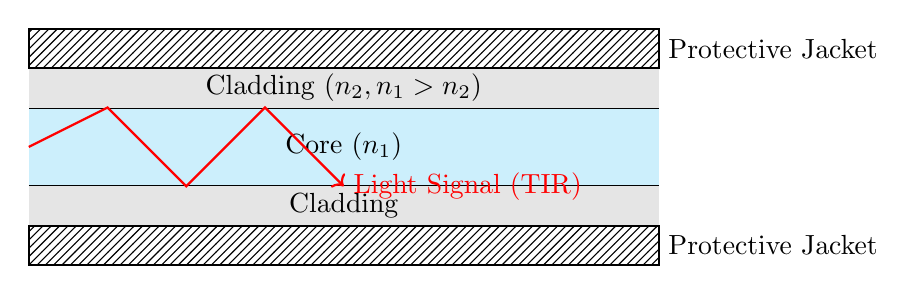
\begin{tikzpicture}
    % Core
    \fill[cyan!20] (0,1) rectangle (8,2);
    \draw[thick] (0,1) -- (8,1);
    \draw[thick] (0,2) -- (8,2);
    \node at (4,1.5) {Core ($n_1$)};
    
    % Cladding
    \fill[gray!20] (0,0.5) rectangle (8,1);
    \fill[gray!20] (0,2) rectangle (8,2.5);
    \draw[thick] (0,0.5) -- (8,0.5);
    \draw[thick] (0,2.5) -- (8,2.5);
    \node at (4,2.25) {Cladding ($n_2, n_1 > n_2$)};
    \node at (4,0.75) {Cladding};
    
    % Jacket
    \draw[thick, pattern=north east lines] (0,0) rectangle (8,0.5);
    \draw[thick, pattern=north east lines] (0,2.5) rectangle (8,3);
    \node[right] at (8,2.75) {Protective Jacket};
    \node[right] at (8,0.25) {Protective Jacket};

    % Light ray
    \draw[red, thick, ->] (0,1.5) -- (1,2) -- (2,1) -- (3,2) -- (4,1);
    \node[red, right] at (4,1) {Light Signal (TIR)};
\end{tikzpicture}
\captionof{figure}{Structure of Optical Fiber}
\end{center}

\textbf{Components:}
\begin{center}
\captionof{table}{Fiber Components}
\begin{tabulary}{\linewidth}{|L|L|L|L|}
\hline
\textbf{Component} & \textbf{Material} & \textbf{Function} & \textbf{Refractive Index} \\ \hline
Core & Glass/Plastic & Light transmission & Higher ($n_1$) \\ \hline
Cladding & Glass & Total internal reflection & Lower ($n_2$) \\ \hline
Jacket & Plastic & Protection & - \\ \hline
\end{tabulary}
\end{center}

\textbf{Working Principle:} Light travels through the core via \keyword{Total Internal Reflection (TIR)} because $n_1 > n_2$.
\end{solutionbox}

\begin{mnemonicbox}
\mnemonic{Core Cladding Jacket, Higher Lower Protection}
\end{mnemonicbox}

\questionmarks{4(B)(2)}{4}{List applications of LASER in engineering and medical field.}

\begin{solutionbox}
\textbf{Engineering Applications:}
\begin{itemize}
    \item \keyword{Cutting and welding}: Precision metal cutting.
    \item \keyword{3D printing}: Laser sintering.
    \item \keyword{Measurement}: Distance measuring and surveying (LIDAR).
    \item \keyword{Communication}: Optical fiber systems.
    \item \keyword{Material processing}: Surface hardening.
    \item \keyword{Barcode scanning}: Retail and inventory.
\end{itemize}

\textbf{Medical Applications:}
\begin{itemize}
    \item \keyword{Surgery}: Precise tissue cutting (bloodless surgery).
    \item \keyword{Eye treatment}: LASIK corrective surgery.
    \item \keyword{Cancer treatment}: Tumor destruction.
    \item \keyword{Diagnostics}: Spectroscopy.
    \item \keyword{Dentistry}: Cavity treatment.
    \item \keyword{Skin treatment}: Cosmetic procedures (hair removal).
\end{itemize}
\end{solutionbox}

\begin{mnemonicbox}
\mnemonic{Engineering: Cut Weld Measure Communicate, Medical: Surgery Eye Cancer Diagnose}
\end{mnemonicbox}

\questionmarks{4(B)(3)}{4}{Explain P-type and N-type semiconductors.}

\begin{solutionbox}
\begin{center}
\captionof{table}{N-type vs P-type Semiconductors}
\begin{tabulary}{\linewidth}{|L|L|L|}
\hline
\textbf{Property} & \textbf{N-type} & \textbf{P-type} \\ \hline
Dopant & Phosphorus, Arsenic (Pentavalent) & Boron, Aluminum (Trivalent) \\ \hline
Majority Carriers & Electrons & Holes \\ \hline
Minority Carriers & Holes & Electrons \\ \hline
Charge & Electrically Neutral & Electrically Neutral \\ \hline
Formation & Donor impurity adds electrons & Acceptor impurity creates holes \\ \hline
\end{tabulary}
\end{center}
Both types are formed by \keyword{doping} intrinsic semiconductors (like Si or Ge) with specific impurities to increase conductivity.
\end{solutionbox}

\begin{mnemonicbox}
\mnemonic{N-type Negative electrons, P-type Positive holes}
\end{mnemonicbox}

\questionmarks{5(A)}{6}{Attempt any two}

\questionmarks{5(A)(1)}{3}{Classify conductors, semiconductors and insulators based on energy band gap.}

\begin{solutionbox}
\begin{center}
\captionof{table}{Material Classification}
\begin{tabulary}{\linewidth}{|L|L|L|}
\hline
\textbf{Material} & \textbf{Energy Band Gap} & \textbf{Characteristics} \\ \hline
Conductor & No gap (0 eV) & Valence and conduction bands overlap \\ \hline
Semiconductor & Small gap (1-3 eV) & Moderate band gap \\ \hline
Insulator & Large gap (>3 eV) & Wide band gap \\ \hline
\end{tabulary}
\end{center}

\textbf{Energy Band Diagram:}
\begin{center}
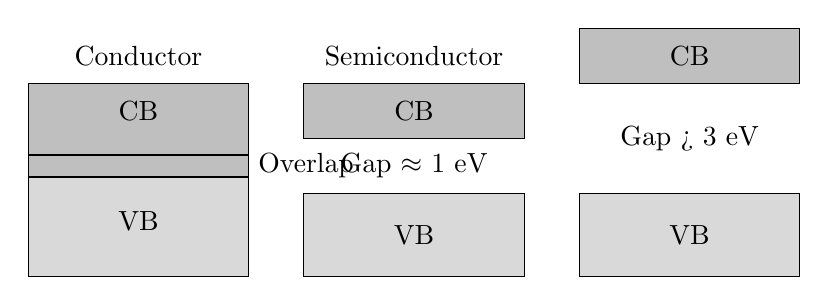
\begin{tikzpicture}[scale=0.7]
    % Conductor
    \node at (2,4) {Conductor};
    \fill[gray!30] (0,0) rectangle (4,2.2); % VB
    \fill[gray!50] (0,1.8) rectangle (4,3.5); % CB overlap
    \draw (0,0) rectangle (4,2.2);
    \draw (0,1.8) rectangle (4,3.5);
    \node at (2,1) {VB};
    \node at (2,3) {CB};
    \node[right] at (4,2) {Overlap};

    % Semiconductor
    \node at (7,4) {Semiconductor};
    \fill[gray!30] (5,0) rectangle (9,1.5); % VB
    \fill[gray!50] (5,2.5) rectangle (9,3.5); % CB
    \draw (5,0) rectangle (9,1.5);
    \draw (5,2.5) rectangle (9,3.5);
    \node at (7,0.75) {VB};
    \node at (7,3) {CB};
    \node at (7,2) {Gap $\approx$ 1 eV};

    % Insulator
    \node at (12,4) {Insulator};
    \fill[gray!30] (10,0) rectangle (14,1.5); % VB
    \fill[gray!50] (10,3.5) rectangle (14,4.5); % CB
    \draw (10,0) rectangle (14,1.5);
    \draw (10,3.5) rectangle (14,4.5);
    \node at (12,0.75) {VB};
    \node at (12,4) {CB};
    \node at (12,2.5) {Gap > 3 eV};
\end{tikzpicture}
\captionof{figure}{Energy Band Diagrams}
\end{center}
\end{solutionbox}

\begin{mnemonicbox}
\mnemonic{No gap Conducts, Small gap Semi, Large gap Insulates}
\end{mnemonicbox}

\questionmarks{5(A)(2)}{3}{Explain OR and AND logic gates with necessary truth table.}

\begin{solutionbox}
\begin{center}
\begin{tabular}{cc}
\begin{minipage}{0.45\linewidth}
\begin{center}
\textbf{OR Gate}
\[ Y = A + B \]
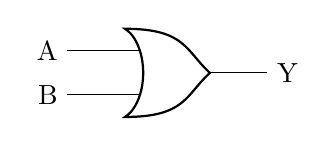
\begin{tikzpicture}
    \node[or port] (or) at (0,0) {};
    \draw (or.in 1) -- ++(-0.5,0) node[left] {A};
    \draw (or.in 2) -- ++(-0.5,0) node[left] {B};
    \draw (or.out) -- ++(0.5,0) node[right] {Y};
\end{tikzpicture}

\begin{tabular}{|c|c|c|}
\hline
A & B & Y \\ \hline
0 & 0 & 0 \\ \hline
0 & 1 & 1 \\ \hline
1 & 0 & 1 \\ \hline
1 & 1 & 1 \\ \hline
\end{tabular}
\end{center}
\end{minipage}
&
\begin{minipage}{0.45\linewidth}
\begin{center}
\textbf{AND Gate}
\[ Y = A \cdot B \]
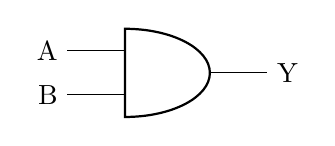
\begin{tikzpicture}
    \node[and port] (and) at (0,0) {};
    \draw (and.in 1) -- ++(-0.5,0) node[left] {A};
    \draw (and.in 2) -- ++(-0.5,0) node[left] {B};
    \draw (and.out) -- ++(0.5,0) node[right] {Y};
\end{tikzpicture}

\begin{tabular}{|c|c|c|}
\hline
A & B & Y \\ \hline
0 & 0 & 0 \\ \hline
0 & 1 & 0 \\ \hline
1 & 0 & 0 \\ \hline
1 & 1 & 1 \\ \hline
\end{tabular}
\end{center}
\end{minipage}
\end{tabular}
\end{center}
\end{solutionbox}

\begin{mnemonicbox}
\mnemonic{OR: Any high makes high, AND: All high makes high}
\end{mnemonicbox}

\questionmarks{5(A)(3)}{3}{Describe the use of Zener diode as a voltage regulator.}

\begin{solutionbox}
\textbf{Circuit Diagram:}
\begin{center}
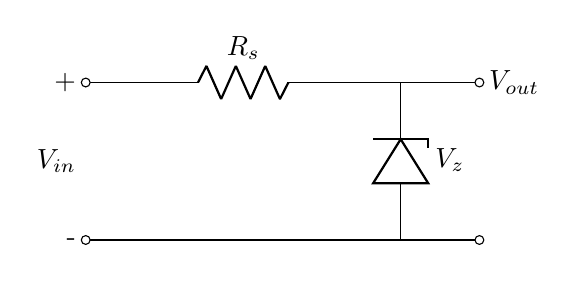
\begin{tikzpicture}
    \draw (0,2) to[short, o-] (1,2)
        to[R, l=$R_s$] (3,2) -- (4,2)
        to[short, -o] (5,2) node[right] {$V_{out}$};
    \draw (4,2) to[zD, l=$V_z$, invert] (4,0);
    \draw (0,0) to[short, o-o] (5,0);
    \node[left] at (0,1) {$V_{in}$};
    \node[left] at (0,2) {+};
    \node[left] at (0,0) {-};
\end{tikzpicture}
\captionof{figure}{Zener Voltage Regulator}
\end{center}

\textbf{Working Principle:}
\begin{itemize}
    \item \keyword{Reverse Bias}: Zener diode is connected in reverse bias.
    \item \keyword{Breakdown}: When $V_{in}$ exceeds Zener voltage $V_z$, the diode conducts deeply in breakdown region.
    \item \keyword{Regulation}: Voltage across Zener remains constant ($V_z$) despite changes in input voltage or load current.
    \item \keyword{Series Resistor} ($R_s$): Limits the current to protect the Zener diode.
\end{itemize}
\end{solutionbox}

\begin{mnemonicbox}
\mnemonic{Zener Zealously maintains Voltage despite Variations}
\end{mnemonicbox}

\questionmarks{5(B)}{8}{Attempt any two}

\questionmarks{5(B)(1)}{4}{Explain full wave rectifier with necessary circuit and draw input and output waveforms.}

\begin{solutionbox}
\textbf{Circuit Diagram (Center-Tapped):}
\begin{center}
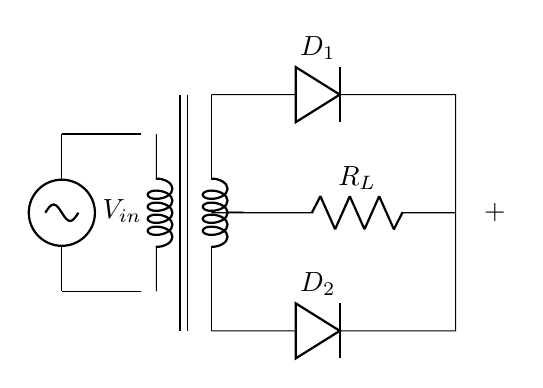
\begin{tikzpicture}
    % Center Tap Rectifier
    \draw (0,2) to[sinusoidal voltage source, l=$V_{in}$] (0,0);
    \draw (0,2) -- (1,2); \draw (0,0) -- (1,0); 
    % Transformer representation simplified
    \draw (1.5,2.5) -- (1.5,-0.5); \draw (1.6,2.5) -- (1.6,-0.5); % core
    \draw (1.2,2) to[L] (1.2,0); % Primary
    \draw (1.9,2.5) to[L] (1.9,-0.5); % Secondary
    % Diodes
    \draw (1.9,2.5) -- (2.5,2.5) to[D, l=$D_1$] (4,2.5) -- (5,2.5) -- (5,1);
    \draw (1.9,-0.5) -- (2.5,-0.5) to[D, l=$D_2$] (4,-0.5) -- (5,-0.5) -- (5,1);
    % Load
    \draw (1.9,1) -- (2.5,1) -- (2.5,1) to[R, l=$R_L$] (5,1);
    % Output
    \node at (5.5,1) {$+$}; \node at (2.2,1) {$-$};
\end{tikzpicture}
\captionof{figure}{Full Wave Rectifier}
\end{center}

\textbf{Waveforms:}
\begin{center}
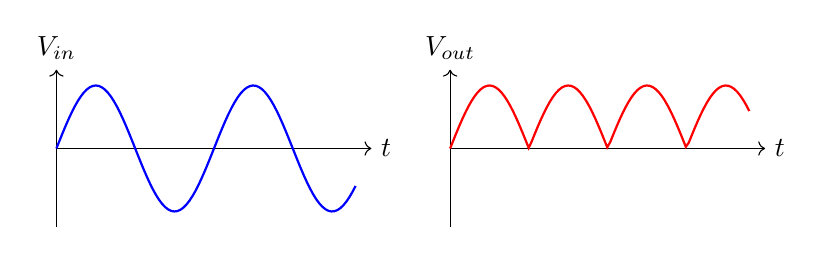
\begin{tikzpicture}
    % Input
    \draw[->] (0,0) -- (4,0) node[right] {$t$};
    \draw[->] (0,-1) -- (0,1) node[above] {$V_{in}$};
    \draw[blue, thick] plot[domain=0:3.8, samples=100] (\x, {0.8*sin(3.14*\x r)});
    
    % Output
    \draw[->] (5,0) -- (9,0) node[right] {$t$};
    \draw[->] (5,-1) -- (5,1) node[above] {$V_{out}$};
    \draw[red, thick] plot[domain=5:8.8, samples=100] (\x, {0.8*abs(sin(3.14*(\x-5) r))});
\end{tikzpicture}
\captionof{figure}{Input and Output Waveforms}
\end{center}
\end{solutionbox}

\begin{mnemonicbox}
\mnemonic{Full wave uses Full cycle, Better efficiency Better output}
\end{mnemonicbox}

\questionmarks{5(B)(2)}{4}{Demonstrate forward and reverse characteristics of P-N junction diode.}

\begin{solutionbox}
\textbf{I-V Characteristic Curve:}
\begin{center}
\begin{tikzpicture}
    \draw[->] (-3,0) -- (3,0) node[right] {$V$};
    \draw[->] (0,-3) -- (0,3) node[above] {$I$};
    % Forward
    \draw[blue, thick] (0,0) -- (0.5,0) to[out=0, in=260] (0.7,0.1) -- (1,2.5);
    \node[right] at (1,2) {Forward Bias};
    \node[below] at (0.7,0) {$0.7V$};
    
    % Reverse
    \draw[red, thick] (0,0) -- (-2, -0.1) -- (-2.2, -2.5);
    \node[left] at (-1.5,-1) {Reverse Bias};
    \node[above] at (-2.2,0) {$V_{BR}$};
\end{tikzpicture}
\captionof{figure}{PN Junction Diode Characteristics}
\end{center}

\textbf{Characteristics:}
\begin{itemize}
    \item \keyword{Forward Bias}: Diode conducts current significantly after cut-in voltage (0.7V for Si).
    \item \keyword{Reverse Bias}: Negligible leakage current until breakdown voltage.
    \item \keyword{Cut-in Voltage}: The voltage at which current starts increasing rapidly.
    \item \keyword{Breakdown}: Sharp increase in reverse current at high reverse voltage.
\end{itemize}
\end{solutionbox}

\begin{mnemonicbox}
\mnemonic{Forward Flow, Reverse Resist}
\end{mnemonicbox}

\questionmarks{5(B)(3)}{4}{Write the principle of LED and explain its construction and working.}

\begin{solutionbox}
\textbf{Principle:} \keyword{Electroluminescence} - Conversion of electrical energy into light energy during carrier recombination.

\textbf{Construction:}
\begin{center}
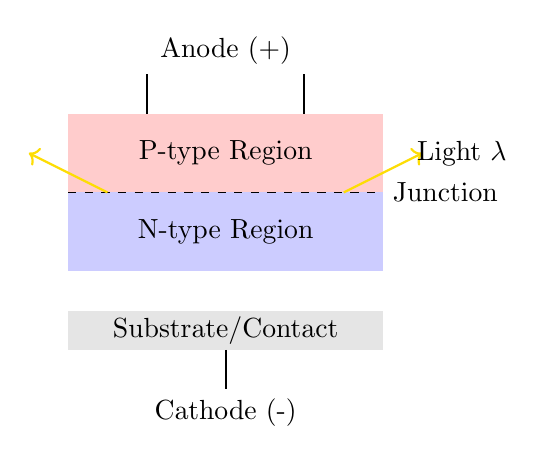
\begin{tikzpicture}
    % Layers
    \fill[red!20] (0,2) rectangle (4,3); \node at (2,2.5) {P-type Region};
    \fill[blue!20] (0,1) rectangle (4,2); \node at (2,1.5) {N-type Region};
    \fill[gray!20] (0,0) rectangle (4,0.5); \node at (2,0.25) {Substrate/Contact};
    
    % Junction
    \draw[dashed] (0,2) -- (4,2); 
    \node[right] at (4,2) {Junction};
    
    % Contacts
    \draw[thick] (1,3) -- (1,3.5); \draw[thick] (3,3) -- (3,3.5);
    \node[above] at (2,3.5) {Anode (+)};
    
    \draw[thick] (2,0) -- (2,-0.5);
    \node[below] at (2,-0.5) {Cathode (-)};
    
    % Light
    \draw[yellow!80!orange, thick, ->] (0.5,2) -- (-0.5,2.5);
    \draw[yellow!80!orange, thick, ->] (3.5,2) -- (4.5,2.5);
    \node at (5,2.5) {Light $\lambda$};
\end{tikzpicture}
\captionof{figure}{LED Construction}
\end{center}

\textbf{Working:}
\begin{itemize}
    \item It operates in \keyword{Forward Bias}.
    \item Electrons from N-region cross into P-region and recombine with holes.
    \item Energy is released in the form of \keyword{photons} (light).
    \item The color depends on the \keyword{band gap} of the semiconductor material (e.g., GaAs for Red).
\end{itemize}
\end{solutionbox}

\begin{mnemonicbox}
\mnemonic{LED: Light Emitting Diode, Electrons and holes Dance to make Light}
\end{mnemonicbox}

\end{document}
